% Replace 'text' below with your text.  Use \citep{Author2016} to add a
% parenthetical citation; use \citet{Author2016} to get a textual cite like
% this: Author (2016).  FS will add the code to insert figures.

\section{Use Consistent Measures}
Properly using measurements is the next critical step in empirical analysis after data collection. It is the crucial stage transforming abstract theoretical concepts to operable data for later empirical tests, which directly affect the internal validity of a study. According to \cite{Hunter2001} and \cite{Hamermesh2007}, internal validity can be divided into two types, statistical replication and scientific replication. Within them, the former particularly relates to the choice and manipulation of measurements. This part of internal validity is assessed ``[w]hen a researcher uses a different sample from the same population to evaluate the same theoretical implication as in the previous study with equivalent construct validity...'' \cite[258]{Morton2010}. To validate a study then requires researchers to conduct tests on theoretically equivalent measures all the way. This is a criterion that should be taken into account not only in the robustness tests but also when the main variables are originally measured in a study, and especially important for studies relying on various data sources which are not collected at the same time by the same design. 

To achieve this criterion, we offer three ``consistencies'' for researchers to check their variable measurements: first, \textit{data collection consistency}. This consistency requires data collected and organized in consistent manner. For instance, when scholars use cross-sectional time-series survey data, their measure of one variable should rely on the same survey questions asking the samples from the same population and coded in the same patterns. This can largely reduce the distortion of the data patterns due to combinations and manipulations (e.g., data format or scale converting) in the measurement construction. Let's illustrate it with an aforementioned example, \cite{Newman2015}. In this study, the authors measured the dependent variable based on data from 2005, 2006, 2007, and 2009 surveys on the US citizens conducted by Pew Research Center. For 2005 and 2006, they used responses from exactly the same question. This strategy guarantees data coming from the \textit{same} organizers, for the \textit{same} question in \textit{same} area, and therefore reduces the risk to violate the inconsistency in the data. Researchers should also be aware that any above ``sames'' singly is not a sufficient condition for measurement consistency. In the previous case, for data from 2007 to 2009, researcher still chose the data from the same organizer and in the same area, but with different questions and coding methods. As shown in the later test, the measurement was no longer adequately consistent. Another example is given by the study of Asia Barometer by \cite{Chu2010}. They found that responses on the same question about the attitude towards democracy did not capture the same aspect of public attitude, but reflected the contextual dependency of the understanding of this concept embedded in various political environments \cite[see, also, ][]{Lu2014a}.

Unfortunately, we may not always enable to hold exactly data collection consistency in researching reality because of the limitations of data availability. Of course, researchers should not let this issue to stop them to sufficiently use all available data (as we suggested in \cref{S:data}), while they have to be more careful when combining and manipulating data. Any inappropriately implement may distort data patterns and introduce serious biases into the analysis. To minimize this risk, researchers are ought to consider at least two issues: \textit{structural consistency} and \textit{method consistency}. Structural consistency no longer releases the requirement in data collection procedure, but still requires data at least being organized (coded) in consistent format. Format differences may lead to more serious issues than researchers commonly expect. A telling example is the measurement debate on challenges of \cite{Przeworski2000} on the classic developmentalist argument about democratization by \cite{Lipset1960}. The former went against the conclusion of the latter by arguing that economic development is not a necessary condition for democratization. Nevertheless, the empirical evidence Przeworski et al. offered relied on a binary measure of degree of democracy as the dependent variable and only income as the main independent variable to measure economic development. This led a serious concern about whether their test truly reject Lipset's theory or just capture a different aspect of the democratization process \cite[not very sure if this citation is adequate][]{Bernhagen2009}. 

Another example is from the previous case of \cite{Newman2015}. As previously mentioned, the measurement of their dependent variable for 2005 and 2006 was created based on responses to which statement comes closest to respondents own view between the following pare of statements: ``Most people who want to get ahead can make it if they're willing to work hard'' or ``Hard work and determination are no guarantee of success for most people.'' If the respondents agreed with the first one, they got 1; if they agreed with the second, then 0. Stated differently, the measure is aggregately binary based on one single question. For the 2007 data, the chosen questions were still about the two statements but, for each statement, there is a 4-scale categorical recorded from ``completely agreed'' to ``completely disagreed.'' When respondents answered completely or mostly agree to \textit{both} statements, they got 1, otherwise, 0. In other words, the variable were measured based on two separate binary questions. For the 2009 data, Newman et al. only used the records for the second statement, even if the question about the first attitude was also asked in the survey as in 2007. For this year, then, respondents only needed to answer ``completely agreed'' or ``mostly agreed'' for the second statement to get 1 in Newman et al. measure of the dependent variable. 

To wrap up, in this example, the authors in this case not only used data with inconsistent format, which we admitted unavoidable in some cases, but also had a \textit{method inconsistency} issue. They used three different methods to convert survey records to binary. This could make the measure very tricky, since the variance in the measure could also be caused or changed due to the applications of multiple methods. 

We tested the difference between the three measurement ways, which confirms the above concern. We creates separated variables based the three measurements Newman et al. used and conducted a comparison. \cref{F:three_measures} presents the results. The plot clearly illustrates how actually different the measures are. Measure 2 is consistently lower than Measure 1 and 3; for 1 and 3, they also follow very different patterns, except for a couple of crosses. Even accounting for the uncertainties in each sampling process, the 95\% confidence intervals did not overlap except in 2012 and only for Measure 1 and 3. In terms of this, creating a variable by combining these three measures is no different to mix three distinctive things together. No one could exactly know what concept is really measured then. In other words, the internal validity has been largely diminished. 

This example illustrates the serious consequence if the structural and the method consistency are not held, and, therefore, the importance to use consistent measures in the social scientific researches. Our suggestion in general is to hold data collection consistency whenever is possible; if the data collection consistency cannot be held, researcher should at least guarantee the structural and method consistencies. They are just released version of the data collection consistency. The difference between the former and the latter lies on the data collection process which we will discuss in the next section.


\begin{figure}[htbp] 
  \caption{Comparing Three Measures of Rejection of Meritocracy Pooled by \citet{Newman2015}}
  \label{F:three_measures}
  \centering
    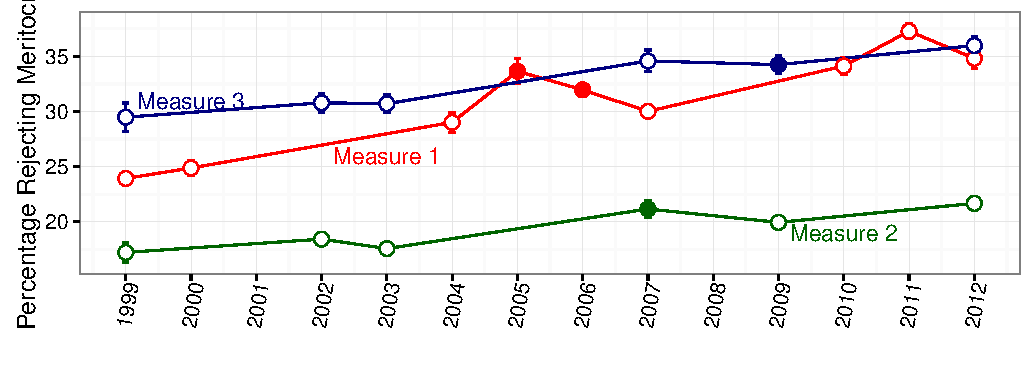
\includegraphics[width=5.25in]{../figures/04_three_measures_whisker.pdf}
  \floatfoot{\emph{Notes}: The analyses presented in Table 1 of \citet[333]{Newman2015} were conducted on pooled observations with the dependent variable, rejection of meritocracy, measured in one of three different ways \citep[see][331]{Newman2015}.  Here, solid circles represent the data used by \citet{Newman2015}; hollow circles represent data in other available Pew surveys. The whiskers are 95\% confidence intervals for each estimates. Plotting the percentage of (weighted) respondents to reject meritocracy by each of these measures reveals that the second measure results in much lower levels of rejection of meritocracy than either of the others and the third often yields considerably higher levels than the first. In light of the evident lack of comparability of these three measures, pooling them into a single analysis cannot be justified.}
\end{figure}

